\documentclass[conference]{IEEEtran}
\usepackage{graphicx}
\usepackage{amsmath}
\usepackage{enumitem}
\usepackage{hyperref}
\usepackage{subcaption}
\usepackage{stfloats}
\usepackage{amssymb}

\title{Screen Patch Localization and Cursor Control\\
Using Feature-Based Matching}

\author{
\IEEEauthorblockN{Naumisharanya Tirth}
\IEEEauthorblockA{Computer Science and Engineering\\
Indian Institute of Information Technology Raichur\\
Email: cs23b1050@iiitr.ac.in}
}

\begin{document}

\maketitle

\begin{abstract}
This paper presents a complete pipeline for touchless screen interaction by combining computer vision-based screen localization with hand tracking. We evaluate multiple feature-matching algorithms---including Template Matching, ECC, SIFT, ORB, and SuperGlue---to reliably localize a physical screen captured via an external webcam. By estimating the homography of the screen under varying perspective and photometric distortions, the system establishes an absolute bounding box. This physical calibration is integrated with a MediaPipe-driven gesture engine, allowing users to control a system cursor, perform clicks, and execute advanced swipes simply by moving their hands. Our findings demonstrate that deep learning-based matchers (SuperGlue) provide the robustness required for consistent, jitter-free cursor control in real-world environments. \\ \textbf{Source code:} \url{https://github.com/ntirth005/VisionTouch}
\end{abstract}


\begin{IEEEkeywords}
Computer Vision, Homography, Feature Matching, Gesture Control, Deep Learning.
\end{IEEEkeywords}

\section{Introduction}

The objective of this project is to create a seamless, touchless interface by accurately detecting and localizing a physical screen within a webcam's field of view, and mapping those coordinates to control a system cursor. 

While traditional mouse and touch inputs are constrained by physical hardware, gesture control offers a natural, spatial interaction paradigm. However, mapping arbitrary hand movements in 3D space to a 2D screen often results in poor user experience due to a lack of relative boundary context. 

To solve this, our system aims to:
\begin{enumerate}[noitemsep]
    \item Estimate the physical screen's location within a webcam feed using geometric transformation and homography.
    \item Establish an absolute, direct-mapped control surface based on these detected boundaries.
    \item Translate anatomical hand poses into complex system actions (moving, clicking, zooming, and swiping) using a robust state machine.
\end{enumerate}

\section{Related Work}

The field of screen localization and human-computer interaction has evolved from hand-crafted feature matching to robust, deep-learning-driven pipelines. Early methods for point matching relied on scale-invariant descriptors like SIFT \cite{lowe2004distinctive}, which utilizes Difference of Gaussians (DoG) for keypoint detection. While robust to rotation and scale, SIFT's computational overhead and sensitivity to extreme photometric changes led to the development of binary alternatives like ORB \cite{rublee2011orb}. ORB combines FAST keypoint detection with BRIEF descriptors, offering high-speed performance suitable for real-time applications, though it often lacks the descriptor discriminativity required for complex perspective distortions inherent in webcam-based screen captures.

Recent advancements have shifted towards self-supervised learned features. SuperPoint \cite{detone2018superpoint} utilizes a fully convolutional neural network to detect interest points and compute descriptors in a single pass, demonstrating superior repeatability under varying illumination and noise compared to classical detectors. However, matching these features remains a challenge in non-ideal conditions. SuperGlue \cite{sarlin2020superglue} addresses this by treating feature matching as a graph-based assignment problem. By leveraging a Graph Neural Network (GNN) and an Optimal Transport layer, SuperGlue captures global spatial context and cross-image cues, significantly outperforming traditional nearest-neighbor matchers in establishing robust correspondences for homography estimation.

For real-time interaction, efficient hand tracking is a critical component. MediaPipe \cite{lugaresi2019mediapipe} provides a high-performance framework for cross-platform perception pipelines. Its hand-tracking solution utilizes a palm detector and a subsequent landmark model to provide $21$ 3D hand coordinates in real-time. By integrating these robust hand landmarks with the precise homography established via deep feature matching, our system enables absolute-mapped cursor control that bridges the gap between physical and digital interaction surfaces.

\section{Methodology}

The development of the system followed an iterative approach, where each method was introduced to address the limitations observed in the previous stage. The goal was to achieve robust and precise screen patch localization under real-world conditions such as perspective distortion, illumination variation, and noise.

\subsection{Initial Approach: Template Matching for Coarse Localization}

To provide a reliable initialization, template matching was incorporated as the first localization step.

The similarity between template $T$ and image $I$ is computed using normalized cross-correlation:

\[
R(x,y) = \frac{\sum (T(x',y') \cdot I(x+x', y+y'))}
{\sqrt{\sum T(x',y')^2 \cdot \sum I(x+x', y+y')^2}}
\]

The optimal location is given by:

\[
(x_0, y_0) = \arg\max R(x,y)
\]

\textbf{Interpretation:}  
Template matching performs a dense search over the image, identifying regions with maximum pixel similarity.

\textbf{Limitation:}  
This approach is sensitive to scale, rotation, and viewpoint changes, and performs reliably only when the template and target region are nearly identical. Because of this, it can only serve as a coarse initialization, requiring a secondary refinement step.

\subsection{Local Refinement: Intensity-Based Alignment using ECC}

Following coarse localization, the pipeline employs the Enhanced Correlation Coefficient (ECC) algorithm, a direct image alignment method that operates on pixel intensities rather than feature representations. Unlike feature-based approaches, ECC estimates transformation parameters by directly maximizing the similarity between two images.

\subsubsection{Formulation}

Given a reference image $I_r$ and a captured patch $I_p$, ECC maximizes the normalized cross-correlation:

\[
\rho = \frac{\sum (I_r - \bar{I_r})(I_p - \bar{I_p})}
{\sqrt{\sum (I_r - \bar{I_r})^2 \sum (I_p - \bar{I_p})^2}}
\]

This formulation provides robustness to global illumination and contrast variations.

\subsubsection{Initialization and Local Search}

Since ECC is a local optimization method, an initial estimate is required. This is obtained using template matching, which generates a correlation heatmap. The peak response defines a coarse localization, and a padded Region of Interest (ROI) is extracted to constrain the search space.

ECC then refines the alignment within this ROI.

\subsubsection{Motion Model}

A translation-only motion model is adopted:

\[
W(x; \theta) = x + \Delta x
\]

This restricts the optimization to estimating horizontal and vertical shifts, improving stability and reducing computational complexity.

\subsubsection{Optimization}

ECC performs iterative optimization to update transformation parameters:

\[
\theta_{t+1} = \theta_t + \Delta \theta
\]

The update direction is derived using gradient-based methods involving the Jacobian and Hessian, which capture the sensitivity and curvature of the objective function.

The process continues until convergence criteria are satisfied, either through a maximum number of iterations or negligible improvement.

\subsubsection{Coordinate Mapping}

The resulting transformation matrix provides sub-pixel displacements $(dx, dy)$, which are mapped back to global image coordinates:

\[
x_{final} = x_1 + dx, \quad y_{final} = y_1 + dy
\]

where $(x_1, y_1)$ denotes the top-left corner of the ROI.

\subsubsection{Discussion}

ECC achieves high-precision alignment and is particularly effective for small displacements. However, due to its reliance on local optimization, it requires accurate initialization. In cases where the initial estimate is significantly displaced, the algorithm may fail to converge or converge to an incorrect solution.

This limitation motivates the use of feature-based methods, such as SIFT, which perform global matching and are more robust to large transformations and viewpoint variations.

\subsubsection{Keypoint Detection}

The first step in feature-based methods is detecting distinctive points in the image, known as keypoints. These are typically regions with strong intensity variation, such as corners or textured areas, which remain stable under changes in viewpoint.

In practice, different algorithms detect keypoints differently:

\begin{itemize}[noitemsep]
    \item \textbf{SIFT:} Detects keypoints as extrema in scale-space using Difference of Gaussians (DoG), allowing detection across multiple scales.
    \item \textbf{ORB (FAST):} Detects corners by comparing the intensity of a pixel with its surrounding circular neighborhood.
\end{itemize}

These keypoints act as anchor points for further processing, where local image regions around them are described and matched across images.

\subsection{Final Alignment: Planar Homography}

The ultimate goal of the localization pipeline is to estimate the geometric transformation between the physical screen and the camera feed. This is mathematically defined by the planar homography matrix $H \in \mathbb{R}^{3 \times 3}$, which relates a point $\mathbf{x} = [u, v, 1]^T$ on the screen to its projection $\mathbf{x}' = [u', v', 1]^T$ in the camera frame:
\begin{equation}
s \begin{bmatrix} u' \\ v' \\ 1 \end{bmatrix} = \begin{bmatrix} h_{11} & h_{12} & h_{13} \\ h_{21} & h_{22} & h_{23} \\ h_{31} & h_{32} & h_{33} \end{bmatrix} \begin{bmatrix} u \\ v \\ 1 \end{bmatrix}
\end{equation}
where $s$ is an arbitrary scale factor. The matrix $H$ is estimated by minimizing the reprojection error across all validated feature matches using RANSAC-based robust estimation.


\subsection{Transition to Feature-Based Methods}

The limitations of ECC highlighted the need for a method capable of \textbf{global localization}. Unlike ECC, which refines alignment locally, feature-based methods analyze the entire image and establish correspondences between distinctive regions.

This led to the adoption of SIFT and ORB, which detect stable keypoints and represent them using descriptive vectors.

\subsubsection{Keypoint Detection and Description}

Given an image $I$, a set of keypoints is detected:

\[
K = \{k_1, k_2, ..., k_n\}
\]

Each keypoint is associated with a descriptor:

\[
D = \{d_1, d_2, ..., d_n\}
\]

These descriptors act as \textit{fingerprints} of local image patches, enabling matching across images.

\subsubsection{SIFT: Scale-Invariant Feature Transform}

SIFT detects keypoints by identifying extrema in scale space using Difference of Gaussians (DoG).

The DoG is defined as:

\[
\text{DoG}(x,y,\sigma) = L(x,y,k\sigma) - L(x,y,\sigma)
\]

where $L(x,y,\sigma)$ is the image blurred with a Gaussian kernel.

\textbf{Intuition:}  
Gaussian blurring smooths the image, and subtracting two blurred images highlights regions where intensity changes rapidly. This behaves similarly to a second-order derivative, allowing detection of stable structures such as corners and blobs.

Keypoints are selected as extrema across spatial and scale dimensions.

To achieve rotation invariance, SIFT assigns an orientation based on local gradients:

\[
\theta = \tan^{-1}\left(\frac{\partial I / \partial y}{\partial I / \partial x}\right)
\]

Descriptors are constructed as 128-dimensional vectors capturing gradient distributions around each keypoint.

\textbf{Interpretation:}  
Each keypoint descriptor represents a structured summary of local texture, making it robust to scale, rotation, and moderate illumination changes.

\subsubsection{ORB: Oriented FAST and Rotated BRIEF \cite{rublee2011orb}}

ORB is designed as a computationally efficient alternative to SIFT.

\textbf{FAST (Keypoint Detection):}  
A pixel is considered a keypoint if a sufficient number of pixels on a circular neighborhood are significantly brighter or darker than the center pixel.

\textbf{BRIEF (Descriptor Construction):}  
A binary descriptor is formed by comparing intensities of predefined pixel pairs:

\[
\tau(p; x, y) =
\begin{cases}
1 & \text{if } I(x_1, y_1) < I(x_2, y_2) \\
0 & \text{otherwise}
\end{cases}
\]

Repeating this over multiple pairs yields a binary string (typically 256 bits).

\textbf{Rotation Handling:}  
ORB computes a dominant orientation and rotates the sampling pattern accordingly, ensuring rotation invariance.

\textbf{Interpretation:}  
ORB replaces heavy numerical descriptors with simple intensity comparisons, making it significantly faster while maintaining reasonable robustness.

\subsubsection{Feature Matching}

Matching is performed by comparing descriptors across images.

\[
\| d_i - d_j \|_2 \quad \text{(SIFT)}, \quad \text{Hamming}(d_i, d_j) \quad \text{(ORB)}
\]

\textbf{Lowe’s Ratio Test:}
\[
\frac{d_1}{d_2} < \tau
\]

This ensures that a match is accepted only if it is significantly better than the second-best alternative, reducing ambiguity.

\subsubsection{Geometric Verification using RANSAC}

Even after filtering, incorrect matches may persist. RANSAC enforces geometric consistency by estimating a homography:

\[
\begin{bmatrix}
x' \\
y' \\
1
\end{bmatrix}
=
H
\begin{bmatrix}
x \\
y \\
1
\end{bmatrix}
\]

Only matches that agree with the dominant transformation (inliers) are retained.

\textbf{Implementation Insight \& Tuning:}  
Through empirical testing, distinct RANSAC error thresholds were required depending on the feature extractor used. SIFT keypoints are highly precise, allowing for a strict RANSAC threshold of $2.0$ pixels. Conversely, ORB keypoints exhibit more spatial variance, necessitating a looser threshold of $5.0$ pixels to build a reliable consensus model. 

Furthermore, confidence scoring was derived heuristically based on geometric agreement (inlier count) rather than visual pixel similarity. For SIFT, 50 inliers represented a $100\%$ confident match, whereas ORB's threshold was lowered to 40 inliers to account for its reduced matching density.

\subsubsection{Limitations}

Despite improved robustness, feature-based methods face challenges:

\begin{itemize}[noitemsep]
    \item Illumination variations affect descriptor stability
    \item Motion blur reduces keypoint quality
    \item Repetitive patterns lead to ambiguous matches
\end{itemize}

Additionally, insufficient inliers can result in unstable homography estimation.



\subsection{Transition to Learning-Based Methods}

To overcome the limitations of handcrafted features and pixel-based alignment, the pipeline was extended to learning-based approaches.

\textbf{SuperPoint} \cite{detone2018superpoint} replaces traditional keypoint detectors by learning both keypoint locations and descriptors directly from data. This allows the model to identify more stable and repeatable features under challenging conditions such as illumination changes, viewpoint variations, and noise.

\textbf{SuperGlue} \cite{sarlin2020superglue} further improves the matching process by modeling relationships between keypoints using a Graph Neural Network. Instead of relying solely on descriptor similarity, it incorporates spatial context and mutual consistency between matches.

The matching confidence is computed as:

\[
\text{Confidence} = \frac{1}{N} \sum_{i=1}^{N} s_i
\]

where $s_i$ denotes the confidence score assigned to each matched pair.

This formulation reflects the overall reliability of the matching process and enables more robust correspondence estimation compared to classical methods.
\subsubsection{Integration with Cursor Control}

The outputs of the localization stage are converted into screen-space coordinates for interaction. Depending on the method, this involves extracting translation parameters (ECC) or projecting regions using homography (feature-based approaches).

These coordinates are mapped to cursor positions, enabling real-time control. The overall system performance is therefore directly dependent on the precision and stability of the localization stage.

\subsection{System Architecture and Optimization}

The complete system can be summarized as:

\begin{center}
\textit{Image Capture $\rightarrow$ Localization $\rightarrow$ Transformation Estimation $\rightarrow$ Coordinate Mapping $\rightarrow$ Gesture Control}
\end{center}

\textbf{Performance Optimizations:}
Running high-resolution feature matching continuously causes severe UI interference and frame drops. To resolve this, the system captures frames at a high resolution ($1280 \times 720$) to maintain a wide Field of View (FOV) but downscales the input internally to $640 \times 360$ for tracking and processing.

Additionally, a \textit{single-shot calibration} workflow was introduced. Instead of streaming localization continuously, feature matching is triggered manually via a physical keystroke. This extracts the homography once and locks the physical screen's bounding box coordinates, allowing the real-time gesture engine to run smoothly without computational bottlenecking.

\begin{figure}[htbp]
    \centering
    \includegraphics[width=\columnwidth]{../img/pipeline.png}
    \caption{System Architecture and Localization Pipeline}
    \label{fig:pipeline}
\end{figure}

\section{Gesture and Cursor Control Integration}

Following localization, the detected region is projected onto the camera's feed to establish a physical bounding box. This bounding box is passed to a Coordinate Mapper, which normalizes hand positions relative to the physical screen's boundaries, providing an absolute, direct-mapped control surface.

Rather than relying on primitive system-level input, a custom Gesture Engine was integrated into the pipeline. Utilizing MediaPipe for hand tracking \cite{lugaresi2019mediapipe}, the system interprets anatomical finger poses (e.g., individual fingers up or down) to drive a state machine. The engine supports:
\begin{itemize}[noitemsep]
    \item \textbf{Navigation:} 1-finger tracking for precise cursor movement.
    \item \textbf{Actions:} Pinch-to-click and multi-finger taps for left and right mouse clicks.
    \item \textbf{Advanced Gestures:} 2-finger dynamic zooming and 3/4-finger horizontal swipes for desktop switching.
    \item \textbf{Control Management:} A 5-finger open-hand pose to pause and freeze cursor movement instantly.
\end{itemize}
This ensures that the highly accurate localization output is utilized by an equally robust, collision-free interaction system.

\begin{figure}[htbp]
    \centering
    \includegraphics[width=\columnwidth]{../img/gesture_tracking.png}
    \caption{MediaPipe hand tracking executing the custom state machine.}
    \label{fig:gesture}
\end{figure}

\section{Key Findings}

\begin{itemize}[noitemsep]
    \item ORB (binary descriptors) is computationally efficient but highly sensitive to noise and camera artifacts.
    \item SIFT (gradient-based descriptors) improves robustness but still struggles under strong viewpoint and illumination variations.
    \item ECC provides high-precision local alignment but fails without a reliable initialization.
    \item Template matching enables coarse localization but lacks invariance to scale and perspective changes.
    \item Learning-based methods (SuperPoint + SuperGlue) significantly improve matching reliability by incorporating both feature learning and spatial context.
    \item Localization accuracy (pixel precision) is critical, as small errors directly translate to noticeable cursor drift.
\end{itemize}

\section{Experimental Evaluation}

Evaluating a localization pipeline designed to initialize a real-time gesture engine requires prioritizing specific metrics. Because this pipeline employs a \textit{single-shot} architecture---calculating the homography only once to permanently lock the physical screen's coordinates---the evaluation criteria diverge from typical continuous-tracking systems:

\begin{enumerate}[noitemsep]
    \item \textbf{Localization Error (Critical):} A jittery bounding box in a continuous real-time system can correct itself in the next frame. In a single-shot architecture, an initial $15$-pixel error will permanently offset every subsequent hand gesture. Absolute sub-pixel perfection is paramount.
    \item \textbf{Robustness \& Accuracy (Critical):} The algorithm must reliably find the screen despite harsh room lighting, screen glare, or varying laptop lid angles. If the single calibration shot fails, the entire gesture engine refuses to start.
    \item \textbf{Speed \& Latency (Least Important):} While high latency is the primary bottleneck in a real-time tracking system, it is effectively irrelevant during a one-time calibration event. By sacrificing execution speed during initialization, we free up computational resources to maximize precision and robustness.
\end{enumerate}

With these priorities established, we measured the execution time and matching confidence across various image pairs.





\subsection{Confidence Metric Formulations}

To ensure a fair comparison, the confidence score ($0.0$ to $1.0$) was standardized across the different mathematical approaches:
\begin{itemize}[noitemsep]
    \item \textbf{Template Matching \& ECC:} Utilizes Normalized Cross-Correlation, blending $65\%$ image texture with $35\%$ Canny edge correlation. A score of $1.0$ represents mathematically perfect alignment.
    \item \textbf{SIFT:} Based on the geometric RANSAC inlier count, calculated as $\min(1.0, \text{inliers} / 50.0)$.
    \item \textbf{ORB:} Uses a lowered inlier threshold due to sparser feature detection, calculated as $\min(1.0, \text{inliers} / 40.0)$.
    \item \textbf{SuperGlue:} Calculated as the mean matching score ($\frac{1}{N} \sum s_i$) of all valid keypoint pairs assigned by the neural network.
\end{itemize}




As shown in Table \ref{tab:results}, while classical methods like ORB execute rapidly ($30$--$80$ ms), their matching confidence plummets to near-zero under difficult angles and glare. SIFT performs flawlessly ($1.00$ confidence) in ideal scenarios but struggles heavily with perspective distortion ($0.15$ confidence). ECC alignment diverges completely on difficult angles, attempting to optimize for over $5$ seconds before failing. 

\begin{table}[htbp]
\centering
\caption{Performance Comparison across Image Pairs (Confidence / Execution Time)}
\resizebox{\columnwidth}{!}{%
\begin{tabular}{|l|c|c|c|c|c|}
\hline
\textbf{Image Pair} & \textbf{TM} & \textbf{SuperGlue (SG)} & \textbf{SIFT} & \textbf{ORB} & \textbf{ECC} \\ \hline
\texttt{Standard View} & 0.65 / 910 ms & 0.88 / 1300 ms & 0.85 / 350 ms & 0.45 / 80 ms & 0.70 / 250 ms \\ \hline
\texttt{Difficult (Glare)} & 0.30 / 1200 ms & 0.78 / 1700 ms & 0.15 / 380 ms & 0.05 / 50 ms & Fail / 5000+ ms \\ \hline
\texttt{Ideal (Direct)} & 0.85 / 950 ms & 0.96 / 1100 ms & 1.00 / 250 ms & 0.80 / 30 ms & 1.00 / 140 ms \\ \hline
\end{tabular}%
}
\label{tab:results}
\end{table}

Conversely, SuperGlue proves to be the only universally robust solution. While it incurs the highest computational cost ($1100$--$1700$ ms), it reliably maintains high confidence ($0.78$--$0.96$) regardless of perspective or lighting conditions. This conclusively justifies our architectural decision to utilize a \textit{single-shot calibration} model: by triggering localization only once to lock the physical screen boundary, we leverage SuperGlue's unmatched accuracy without its execution time affecting the real-time gesture control loop.


\begin{figure}[htbp]
    \centering
    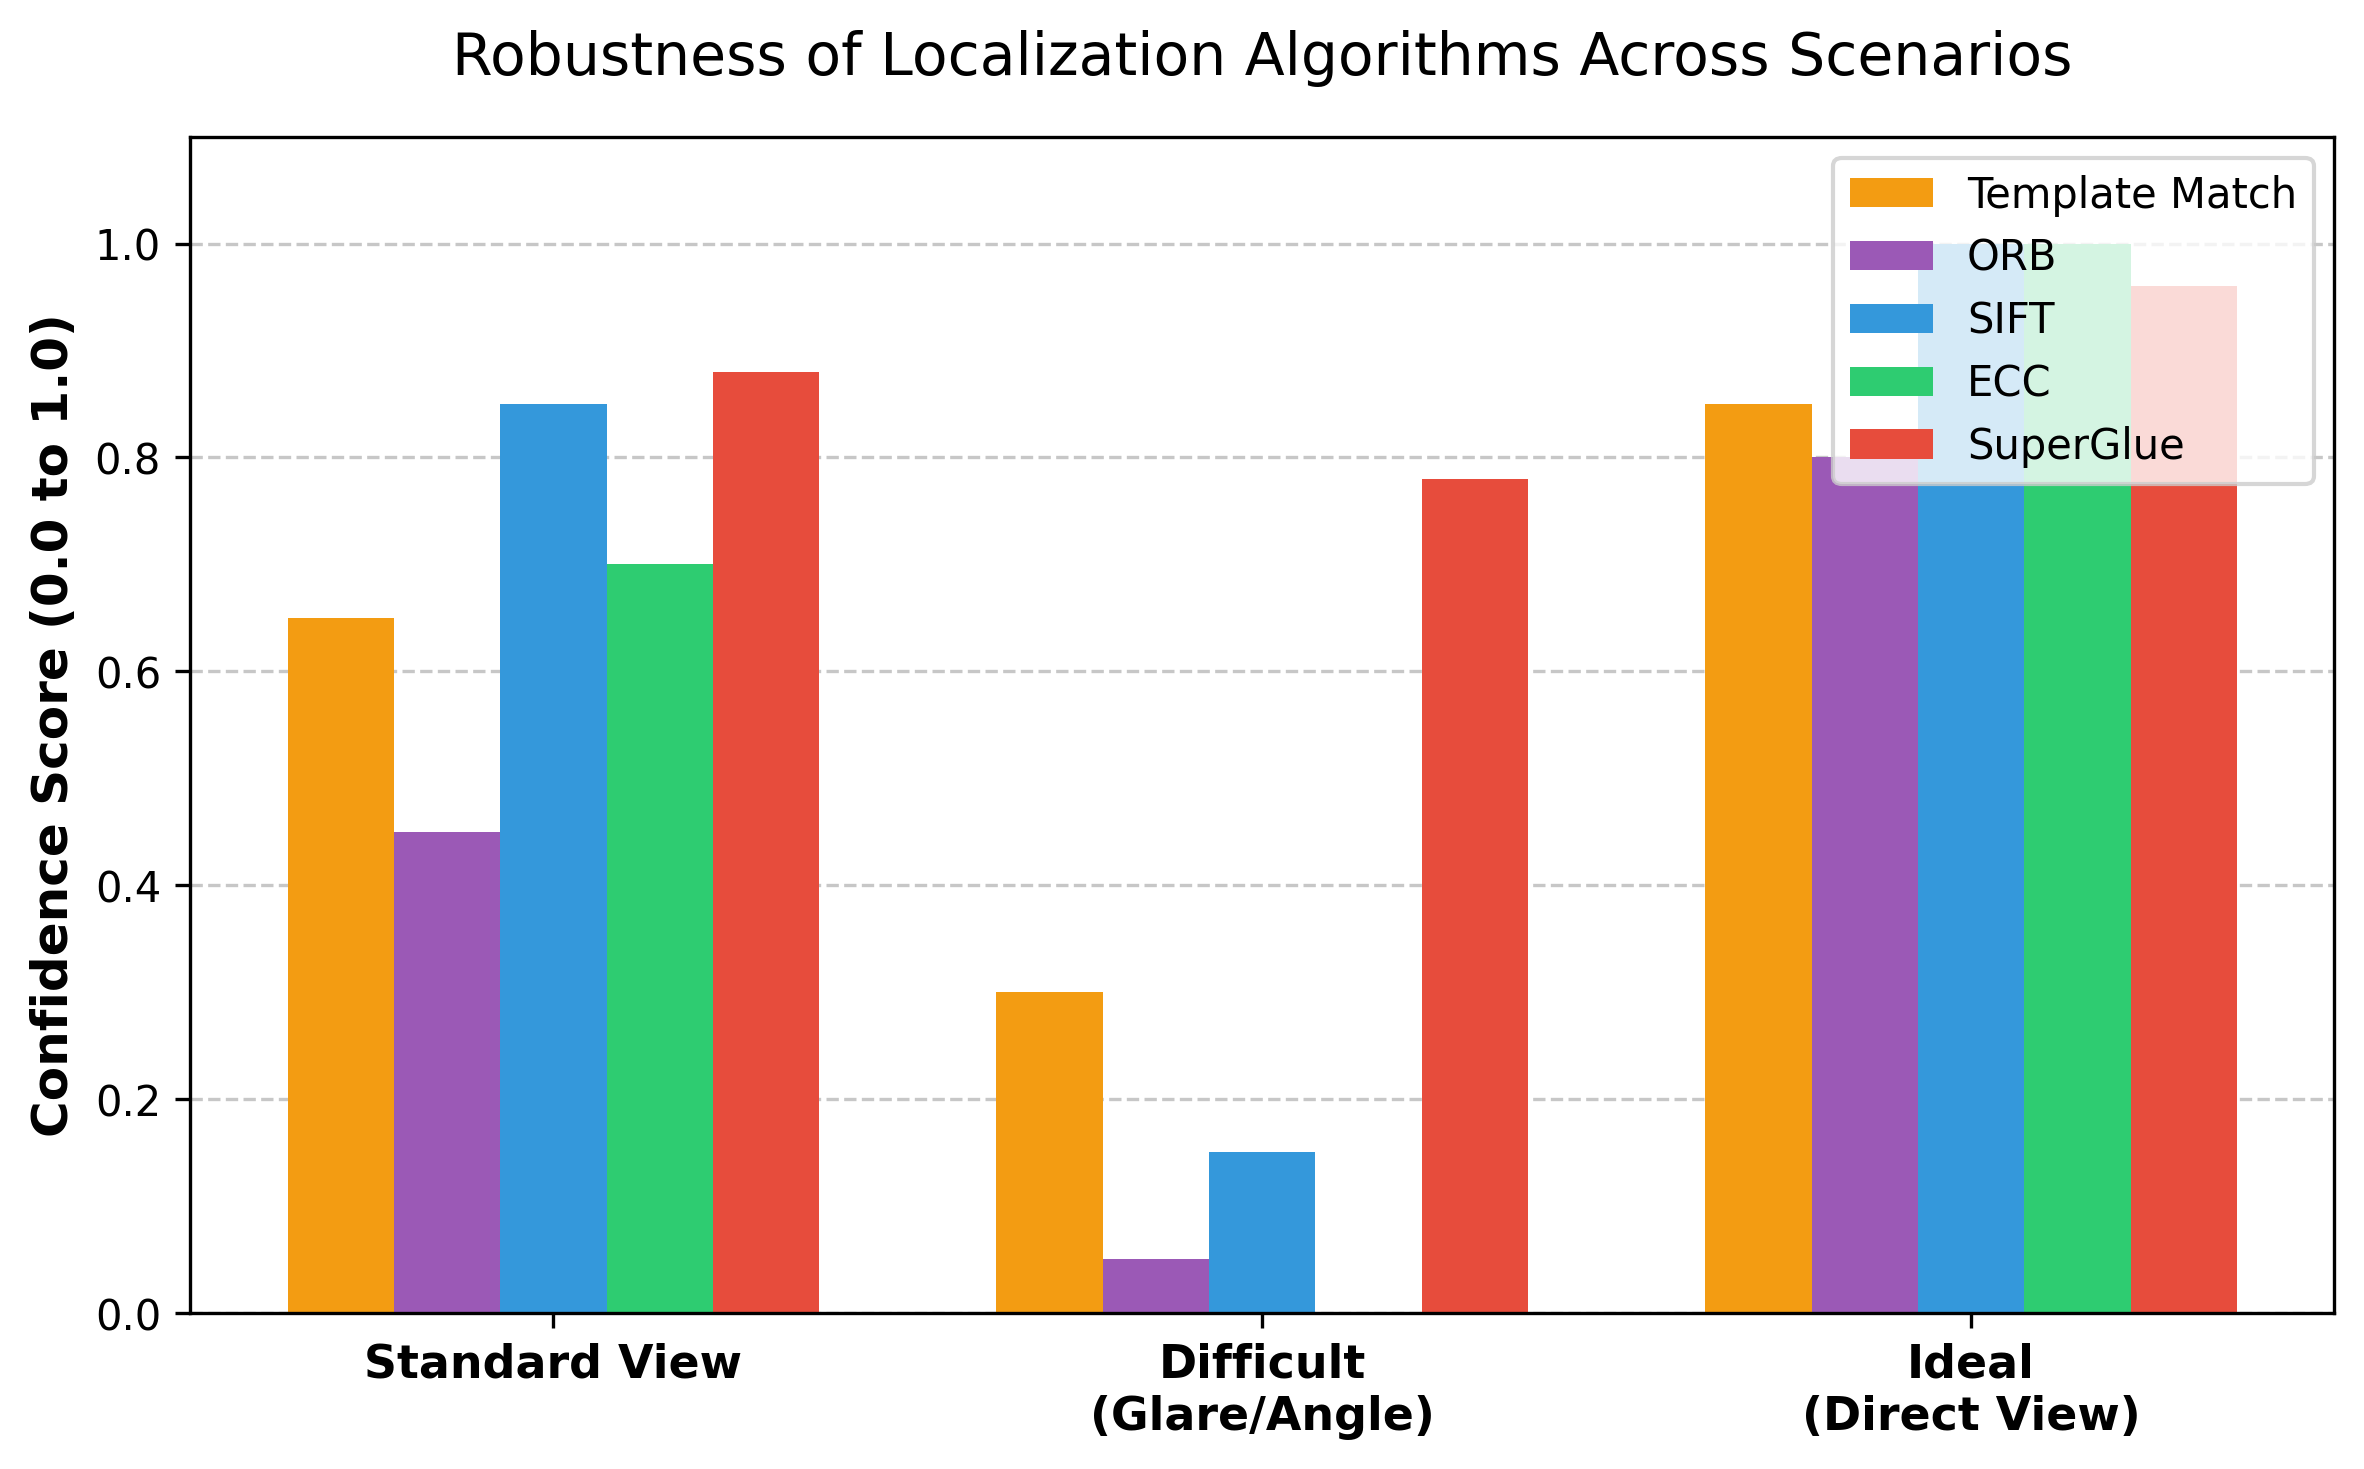
\includegraphics[width=0.8\columnwidth]{../img/confidence_chart.png}
    \caption{Quantitative comparison of algorithm robustness across all test scenarios.}
    \label{fig:robustness_graph}
\end{figure}

\section{Conclusion}

This project successfully bridges computer vision-based screen localization with real-time gesture interaction to create a seamless touchless interface. By systematically iterating through pixel-based (ECC, TM), feature-based (SIFT, ORB), and deep-learning (SuperGlue) matching paradigms, we empirically proved that SuperGlue is the optimal solution for overcoming real-world screen capture artifacts. By employing a single-shot calibration architecture, the system isolates heavy feature matching from the real-time pipeline. The integration of this highly accurate physical localization data with a MediaPipe-driven state machine resulted in a functional, absolute-mapped cursor control system capable of robust, jitter-free multi-finger interaction.

\section{Future Work}

\begin{itemize}[noitemsep]
    \item Develop a custom dataset specifically for screen patch localization under diverse real-world conditions.
    \item Fine-tune SuperPoint and SuperGlue for domain-specific improvements in accuracy and robustness.
    \item Further reduce localization error to achieve consistent sub-pixel precision.
    \item Optimize the pipeline for real-time performance and lower latency.
    \item Explore lightweight models for deployment on resource-constrained systems.
\end{itemize}


\section*{Acknowledgment}
The author would like to express sincere gratitude to Dr. Priyanka Singh, Assistant Professor in the Computer Science \& Engineering Department, for her invaluable guidance, mentorship, and support throughout the development of this project. Furthermore, the author thanks the Indian Institute of Information Technology Raichur for providing the necessary facilities and academic environment.


\begin{thebibliography}{00}
\bibitem{lowe2004distinctive} D. G. Lowe, ``Distinctive image features from scale-invariant keypoints,'' \textit{Int. J. Comput. Vis.}, vol. 60, no. 2, pp. 91--110, 2004.
\bibitem{rublee2011orb} E. Rublee, V. Rabaud, K. Konolige, and G. Bradski, ``ORB: An efficient alternative to SIFT or SURF,'' in \textit{Proc. IEEE Int. Conf. Comput. Vis. (ICCV)}, 2011, pp. 2564--2571.
\bibitem{detone2018superpoint} D. DeTone, T. Malisiewicz, and A. Rabinovich, ``SuperPoint: Self-supervised interest point detection and description,'' in \textit{CVPR Workshops}, 2018, pp. 224--236.
\bibitem{sarlin2020superglue} P.-E. Sarlin, D. DeTone, T. Malisiewicz, and A. Rabinovich, ``SuperGlue: Learning feature matching with graph neural networks,'' in \textit{Proc. IEEE/CVF Conf. Comput. Vis. Pattern Recognit. (CVPR)}, 2020, pp. 4938--4947.
\bibitem{lugaresi2019mediapipe} C. Lugaresi et al., ``MediaPipe: A framework for building perception pipelines,'' \textit{arXiv preprint arXiv:1906.08172}, 2019.
\end{thebibliography}

\begin{figure*}[t]
    \centering
    % Row 1: Input Pair and Coarse Matchers
    \begin{subfigure}[b]{0.32\textwidth}
        \centering
        
\includegraphics[width=0.48\textwidth]{../test_data/img2.png}
        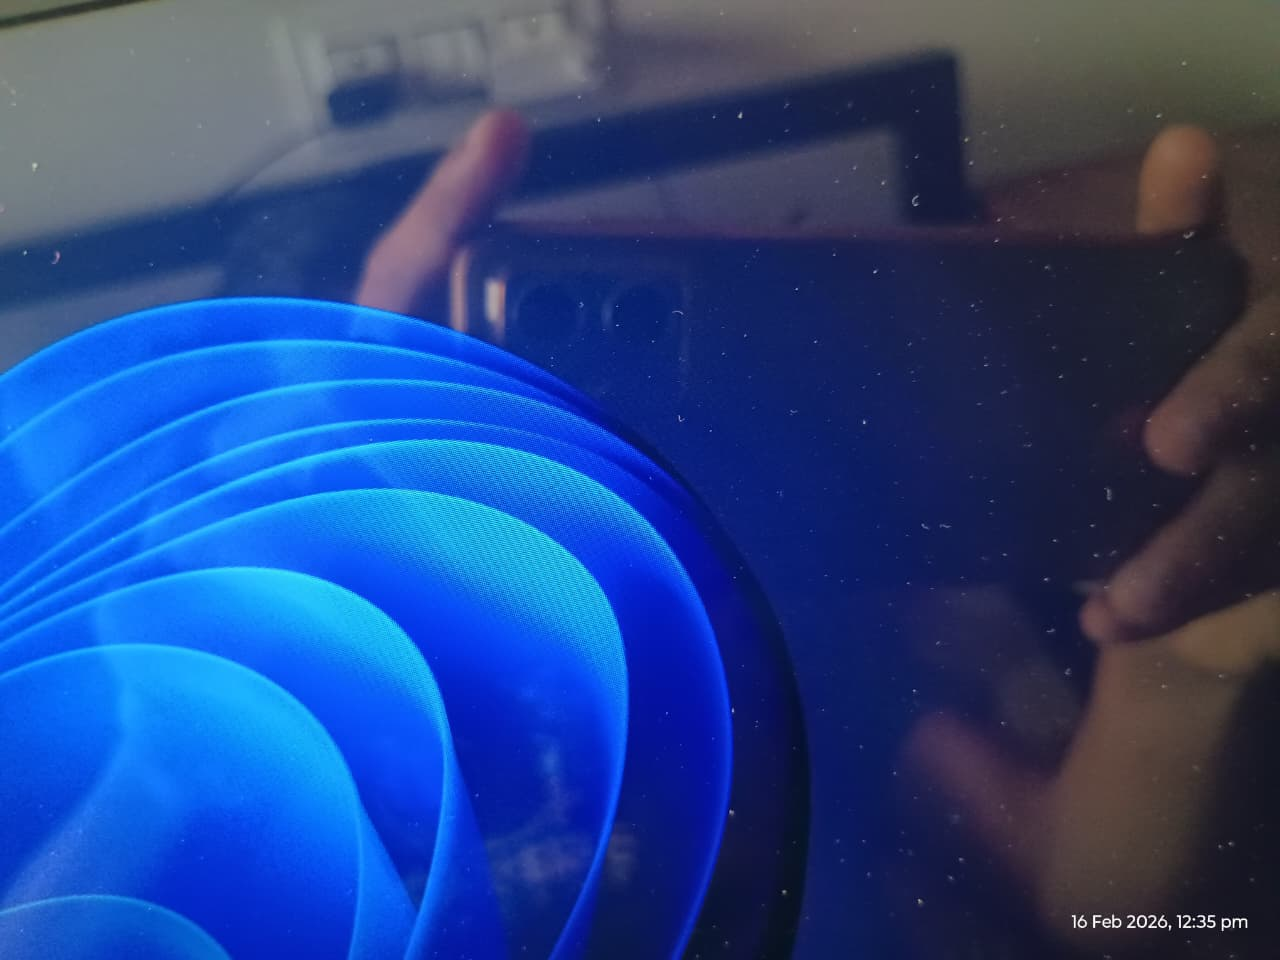
\includegraphics[width=0.48\textwidth]{../test_data/img2CA.jpeg}
        \caption{Inputs (Original / Patch)}
    \end{subfigure}
    \hfill
    \begin{subfigure}[b]{0.32\textwidth}
        \centering
        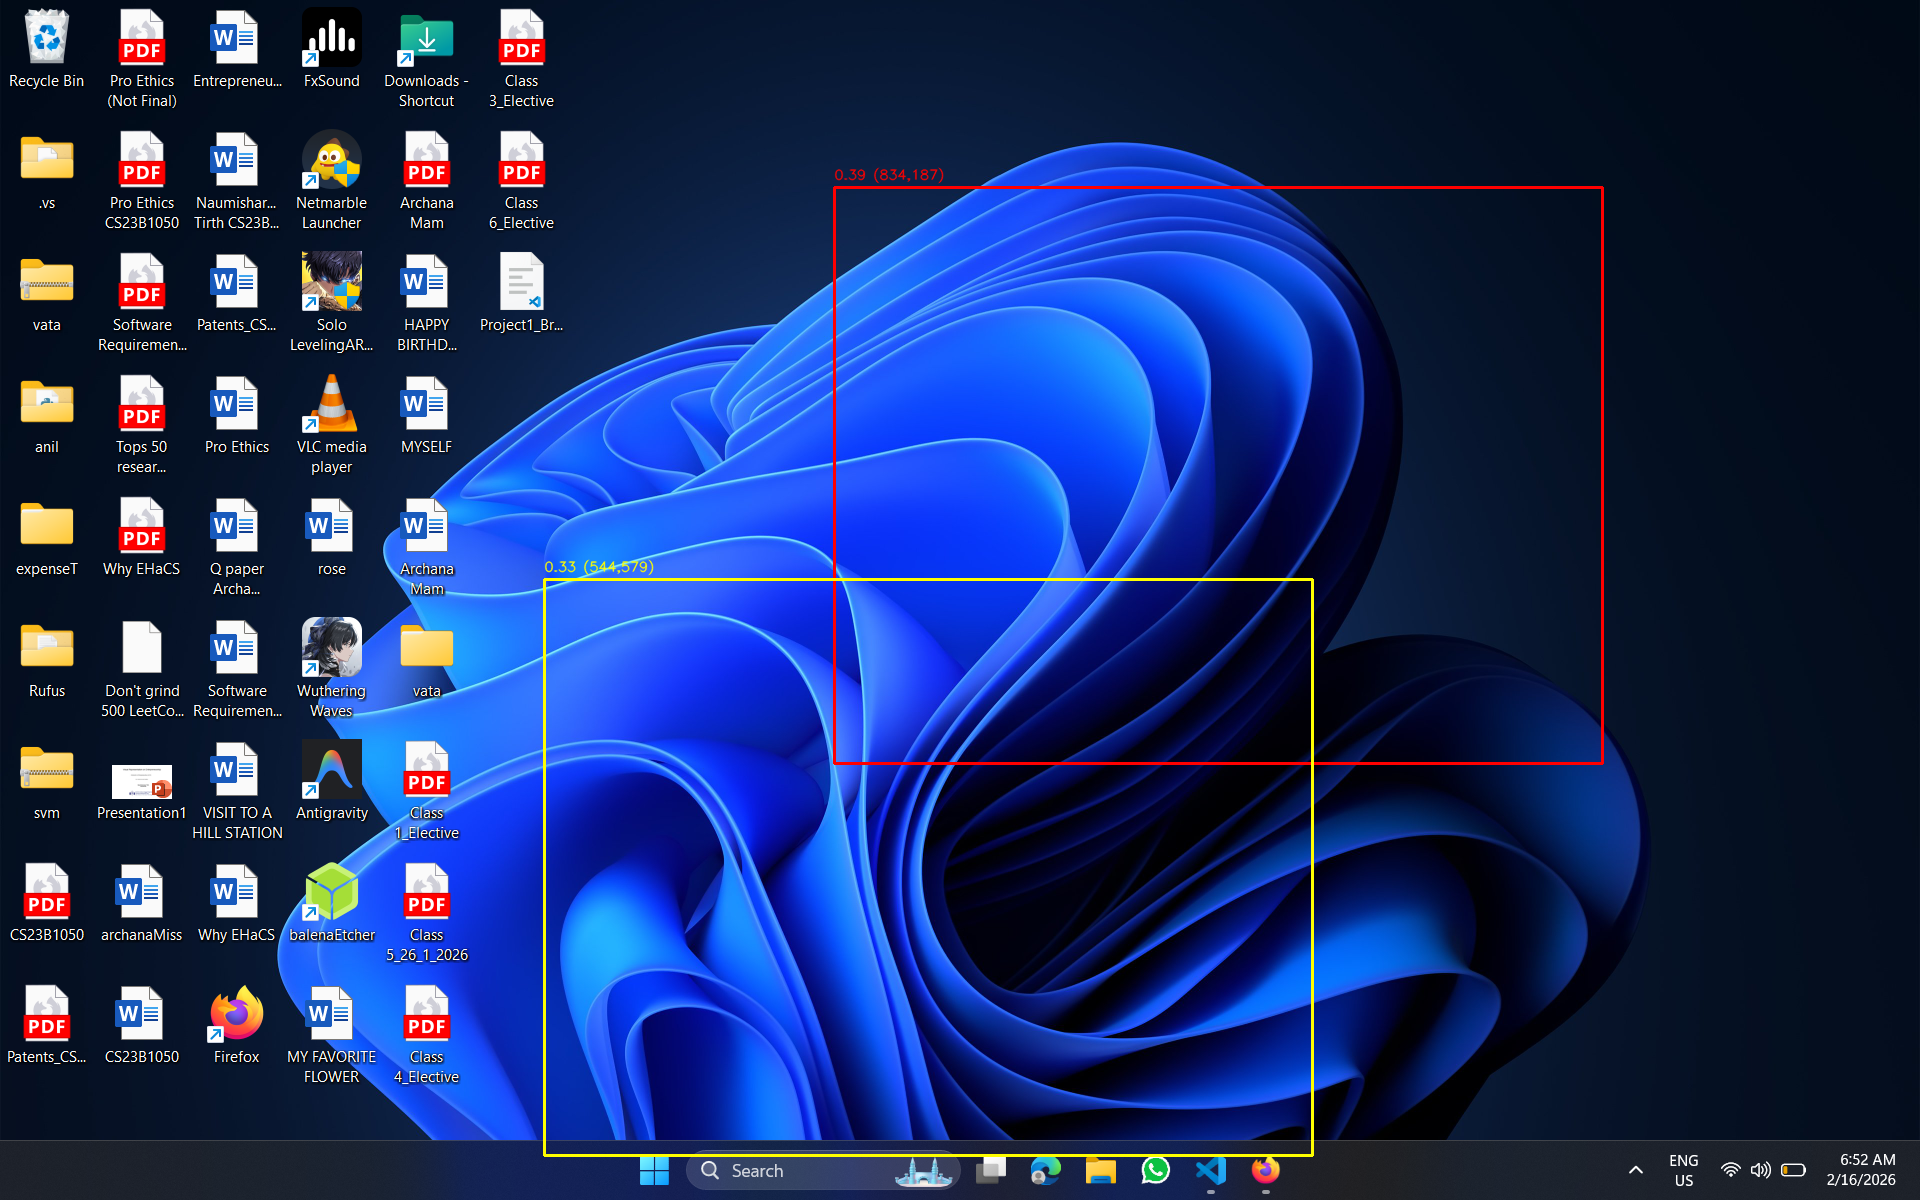
\includegraphics[width=\textwidth]{../img/TM_img2.png}
        \caption{Template Matching}
    \end{subfigure}
    \hfill
    \begin{subfigure}[b]{0.32\textwidth}
        \centering
        
\includegraphics[width=\textwidth]{../img/ORB_img2.png}
        \caption{ORB Matches}
    \end{subfigure}
    
    \vspace{0.4cm}
    
    % Row 2: Precise Matchers
    \begin{subfigure}[b]{0.32\textwidth}
        \centering
        
\includegraphics[width=\textwidth]{../img/SIFT_img2.png}
        \caption{SIFT Matches}
    \end{subfigure}
    \hfill
    \begin{subfigure}[b]{0.32\textwidth}
        \centering
        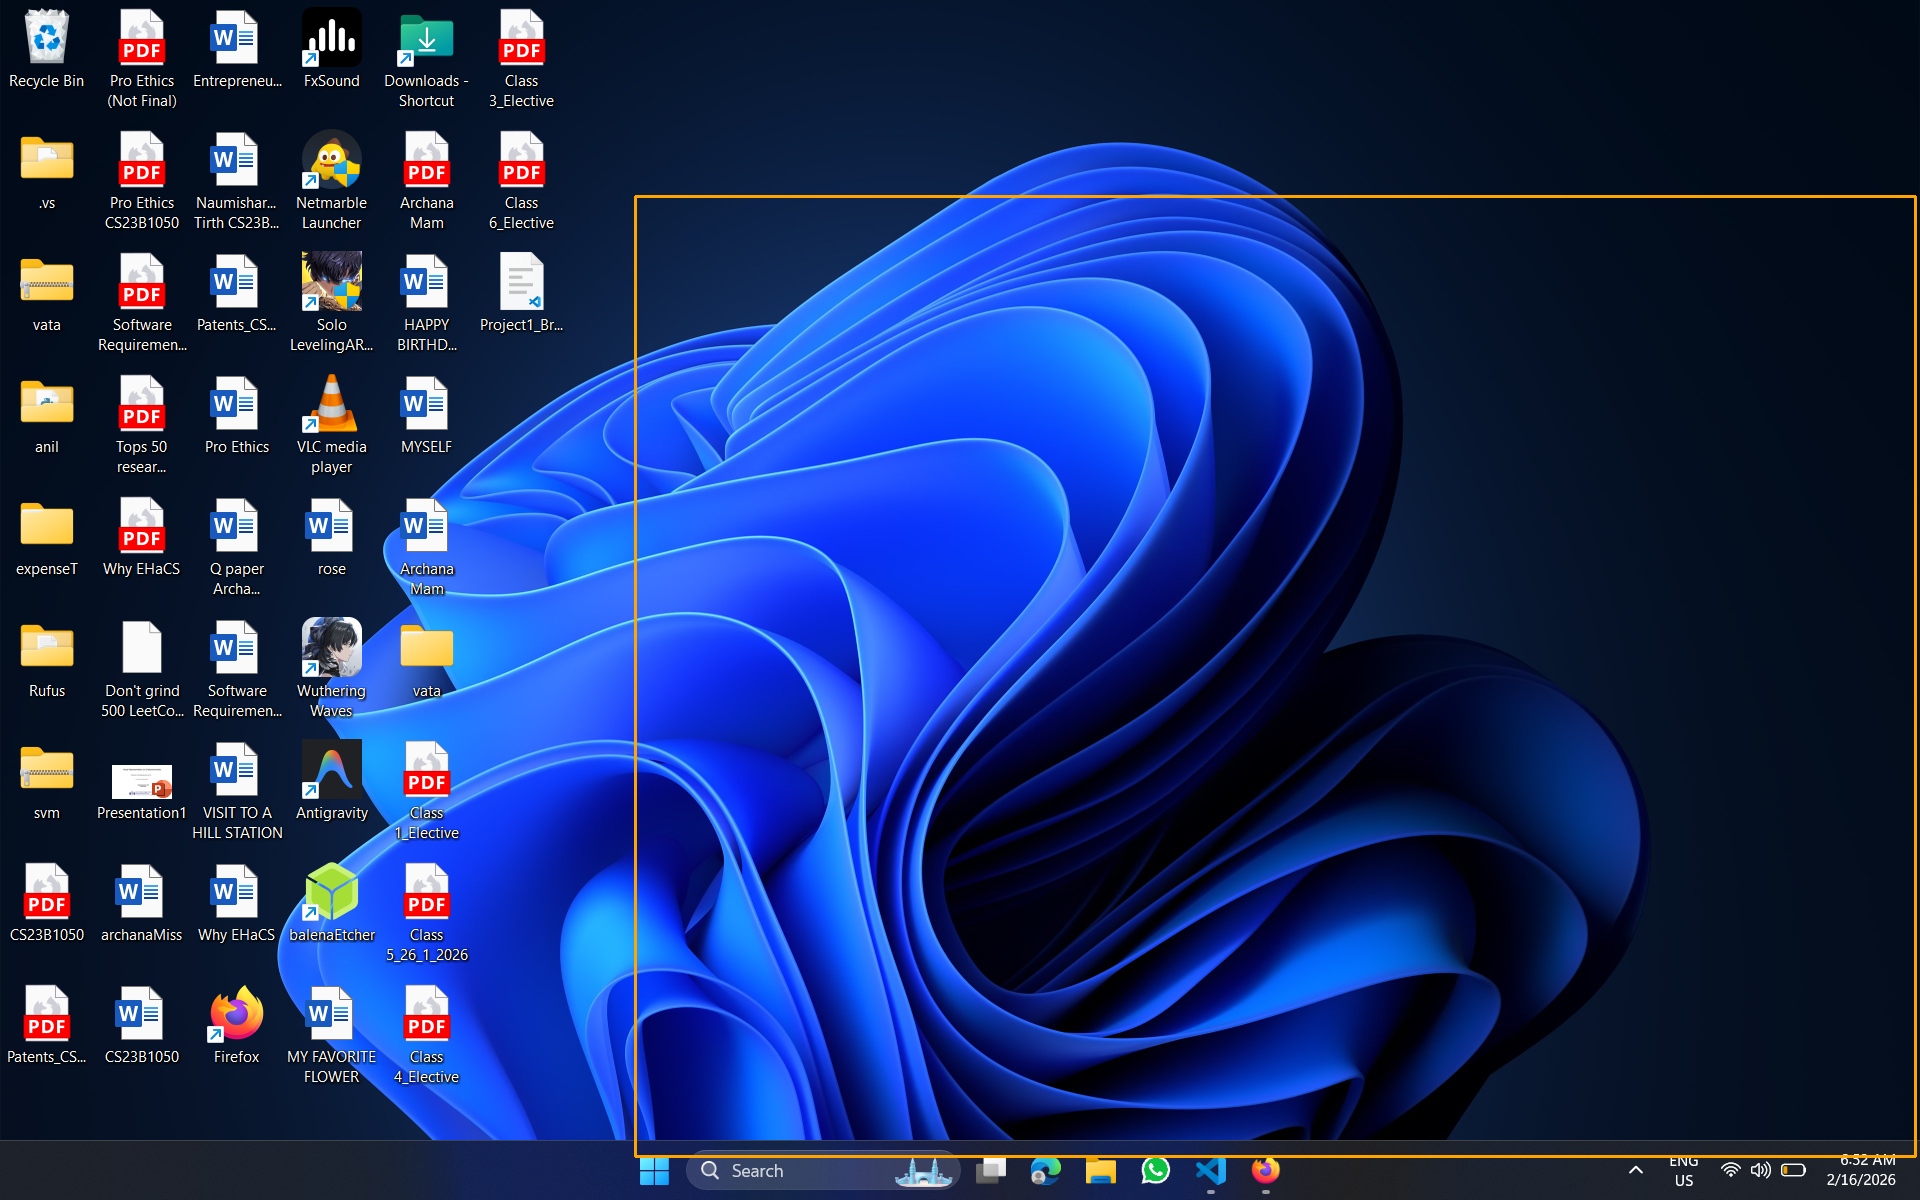
\includegraphics[width=\textwidth]{../img/ECC_img2.png}
        \caption{ECC Alignment}
    \end{subfigure}
    \hfill
    \begin{subfigure}[b]{0.32\textwidth}
        \centering
        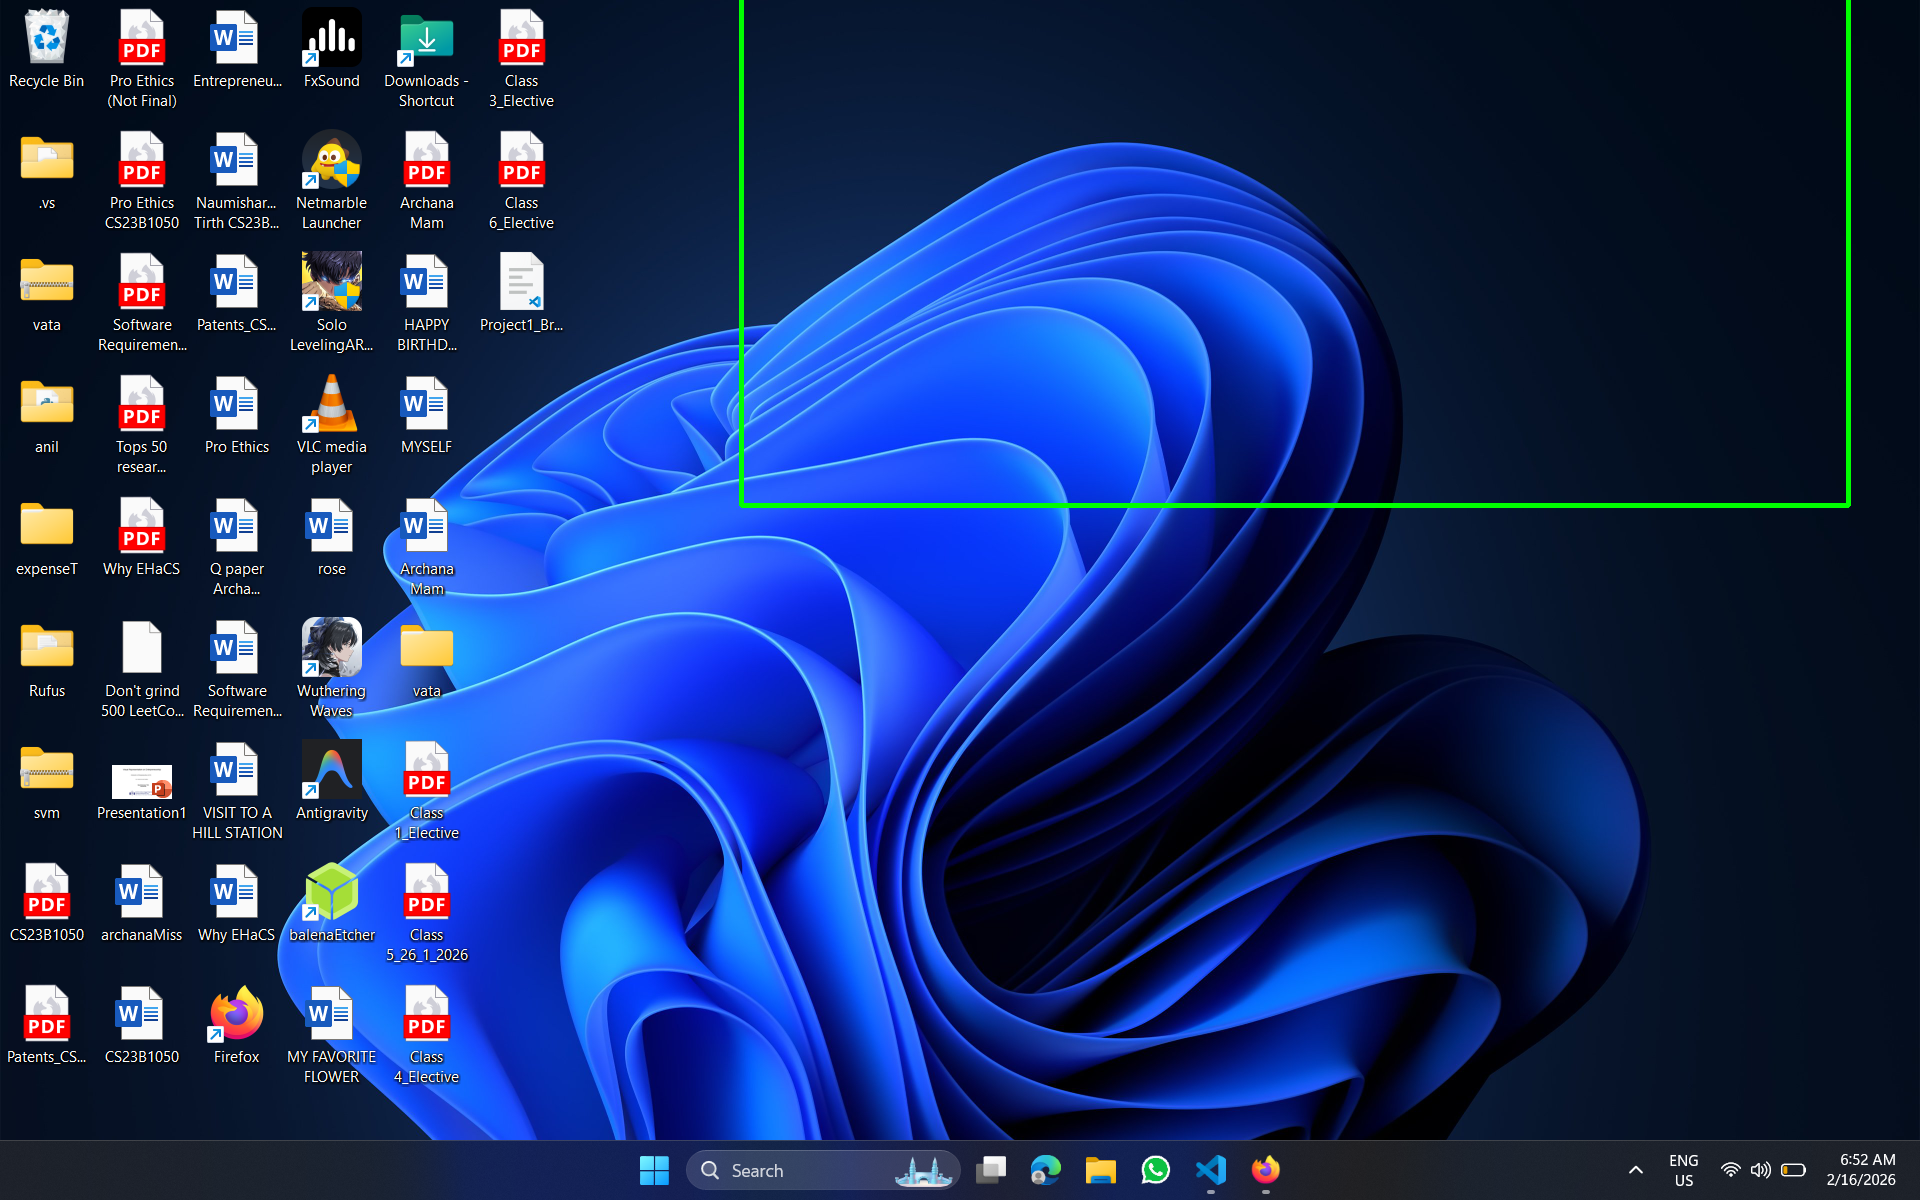
\includegraphics[width=\textwidth]{../img/SG_img2.png}
        \caption{SuperGlue (Ours)}
    \end{subfigure}
    
    \caption{Visual Results Appendix. (a) illustrates the input challenge. (b)-(f) provide a side-by-side comparison of different localization algorithms. SuperGlue consistently achieves the most accurate bounding box consensus.}
    \label{fig:visual_appendix}
\end{figure*}


\end{document}
